\chapter{마치며}

이 긴 문서의 끝에서 다시 만난 독자 여러분!

끝까지 읽어준 여러분께 깊은 감사의 뜻을 전한다.
\vspace{\baselineskip}

지금까지 천문학이라는 바다에 이제 막 배를 띄운 새내기들이 당면하게 될 몇 가지
궁금증을 선정하고, 그에 대한 간략한 도움말을 적어보았다. 사실 기획 초기
단계에서는 서울대학교 천문학과 대학원 생활에 관한 간략한 팁들을 담고 있는 짧은
안내서를 구상하였다. 그러나 주변의 많은 대학원생들간의 토의 끝에, 좀 더 확장된
안내서의 필요성을 느끼게 되었고, 그 기획이 이렇게 커져 방대한 양의 안내서로
거듭나게 되었다. 그러나 이 안내서는 어디까지나 참고자료로 활용되어야지, 이
안내서의 내용을 지나치게 맹신하여서는 안된다. 이 안내서는 간략한 정보만 담고
있을뿐더러, 작성된 이후로 변경된 것들도 있을 것이다. 그렇기 때문에 궁금한 것이
있다면 주저하지 말고 주위 사람들에게 물어보도록 하라.  \vspace{\baselineskip}

\begin{figure}
%  \vspace{-20pt}
  \begin{center}
    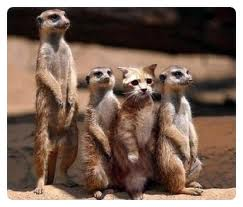
\includegraphics[width=0.48\textwidth]{./Figures/meerkat.jpg}
  \end{center}
  \vspace{-20pt}
  \legend{\textsf{난 누군가. 그리고 여긴 또 어딘가.}}
  \vspace{-10pt}
\end{figure}
한 가지 당부하자면, 질문하는 것을 겁내지 마라. 질문 좀 했다고 해서 선배들이
혼내거나, 이 아이는 왜 이리 멍청한 것일까라고 한탄하거나 하는 일은
없다. (...아마도?) 오히려 이 아이는 선배에게 먼저 다가와주는 귀여운 아이구나라며
이쁨 받을 확률이 더 높다. 모르는 것은 부끄러운 것이 아니다. 오히려 소위
쪽팔릴까봐 모르는 것을 물어보지 못하는 것이야 말로 부끄러운 행동이다.  연구에 막
입문한 사람들이기에, 조금 더 풀어서 써보면, 질문을 많이 하라는 것은 연구를
시작하는데 있어서도 마찬가지이다. 처음 교수님과 면담하거나 팀 미팅에 들어 가보면
신입생 중 십중팔구는 '이게 대체 무슨 소리지?, 나는 누구인가, 그리고 또 여긴
어딘가' 라며 공황상태에 빠지게 될 것인데, 그건 당연한 거다.
\vspace{\baselineskip}

교수님과 대학원생은, 그 분야에 대해서 짧게는 수 학기, 길게는 수 년을 판
사람인데, 이제 갓 연구를 시작한 새내기가 그 사람들 간의 대화를 100\% 이해하는
것이 가당키나 한 일이라고 보는가? 그런 경험은 당신만 겪는 일이 아니니,
의기소침해지거나, 더 나아가 '난 학부 때 너무 놀았나봐 난 글러먹었어'라며 겁먹은
타조마냥 땅에 머리 콕 처박고 자학모드에 들어가거나 하지 않았으면 한다. 그렇게
고뇌와 번민 속에서 허우적거릴 기력과 시간이 있으면 당장 교수님이나 선배를
찾아가서 질문하는 것이 백배천배 낫다. 교수님과 선배님이 신입생 골려주기 위해
어려운 용어를 쓰는 것이 아니다. 단지, 그 사람들은 당신이 못 알아듣는 것을 모르고
평소와 같이 말하고 있었을 뿐이다. 당신이 못 알아듣는 점에 대해 질문하면 당신이
아직 연구 궤도에 올라오지 못한 신입생이란 것을 그제서야 깨닫고 친절히 지금 무슨
이야기를 하고 있는 것인지 풀어서 설명해주실 것이다.  \vspace{\baselineskip}

기초적인 것도 모르는 것 같아서 질문하기에 너무 부끄러워 나중 그냥 따로 찾아보거나
공부하겠다고? 우리 솔직해지자. 그간 중고등학교와 대학교를 합쳐 근 10년 공부했으면
자기 자신에 대해서 좀 알 때가 되지 않았는가. 그 분야를 스스로 찾아서 공부하겠다고?
설령 당신이 칭찬할만한 의지력의 소유자여서 공부하려 하는 시도는 했다고
치자. 교수님들과 선배님들의 이야기는, 연구의 최전선에 있는, 따끈따끈한 것들이
많을텐데, 그 정보가 어디 있는지 어떻게 알 것이며, 어디서 찾을 것인가? 책?
네이버? 위키피디아? 답은 논문이다. 자 그러면, ADS나 arXiv 가서 논문 하나 출력해서
읽어보아라. 아마 abstract, introduction 채 읽기도 전에 논문을 활활 불태우고 싶은
충동에 휩싸일 것이다.  \vspace{\baselineskip}

물론 연구자라면 언젠가는 의무적으로 혼자서 자료를 찾고 모르는 것을 고민하면서
각자의 연구를 개척하며 걸어가는 순간이 오게 된다. 하지만 스스로 일어나 걸을 수
있게 되기까지, 부모님께서 지켜보는 가운데 숱하게 넘어지고 도움 받는 과정이 있다는
것을 잊어서는 안 된다. 대학원 석사 과정으로 입학한다는 건, 연구 인생으로 보면
걸음마를 떼기 시작하는 단계다. 아기가 스스로 걷지 못한다고 그걸 탓하는 사람은
없고, 또 걷지 못한다는 사실에 자괴감에 빠지는 아기는 없다. 대학원 첫 학기는
무엇을 질문해도 다 용서되는 특권을 가진, 연구 인생에서 다시는 오지 않을 가장
소중한 시간이다. 그 소중한 시간을 부디 낭비하지 말고 알차게 사용하길 바란다.
\vspace{\baselineskip}

단, 질문을 할 때, 몇 가지 에티켓 정도는 지키도록 하자.
\begin{enumerate}
\item 자기가 할 수 있는 선에서는 스스로 최선을 다해서 시도해보자. (그렇다고 앞
  문단을 깡그리 잊고, 혼자 이해할 수 없는 분야에 독학한다고 매진하지는 말고...)
  예를 들어, 당신이 처음 리눅스를 접하면 아무것도 모를 것이고 접속하고 계정
  만드는 것까지 선배의 도움을 받아야할 것이다. 하지만, 어느 정도 리눅스를 다룰 수
  있게 된 이후에도 '폴더는 어떻게 만들어요?' '폴더는 어떻게 지워요?' '이거 왜
  복사가 안될까요?' 등, 인터넷 검색만 해봐도 주르륵 뜨는 수준의 질문을 계속하는
  것도 예의 있는 행동은 아니다.
\item 질문은 최대한 구체적으로 하자. 물론, 아무런 지식 기반이 없으면, 자기가 뭘
  모르는지도 확실히 모를 수도 있다는 것은 이해하지만, 두루뭉실한 질문은 선배가
  들었을 때 친절히 답변해주고 싶어도 '어쩌라고?'라는 생각이 들기 마련이다.  예를
  들어 밑도 끝도 없이 '측광 어떻게 해요?' 라고 물어보면 선배는 그저 '잘' 이라고
  밖에 대답해줄 수밖에 없다. 그렇기에 '선생님께서 어떤어떤 일을 저에게 시키려고
  하는 것 같습니다. 그런데 홈페이지 갔는데 자료를 어떻게 받는지 잘
  모르겠네요. 그리고 측광하는 건 어떤 프로그램을 써야하는가요?' 라고 질문을
  구체적으로 하자.
\item 한 선배에게 집중질문 하지 말자. 앞서 질문 좀 했다고 뭐라하는 선배 없다고
  했지만, 어디까지나 '인간적인' 범위 내에서의 이야기지, 하루 종일 하나부터 열까지
  한 선배만 붙잡고 있다면, 그 선배도 사람인 이상 짜증이 날 수 밖에 없다.  (특별히
  자기에게 신경을 많이 써주는 선배분께는 감사하다고 캔커피 하나 정도 사드리는
  센스를 발휘하는 것도 좋다)
\end{enumerate}
\vspace{\baselineskip}

마지막으로, 사족을 덧붙이면 선배 및 동기와 친해지라는 것이다. 연구 생활 역시 사회
생활의 하나이고, 연구자들 간의 교류는 연구자의 중요한 덕목 중 하나이다. 실제로
선후배 동기들 간의 대화로부터 연구 내외적인 면에서 많은 조언 및 아이디어를
주고받을 수 있다. 자신은 백년에 한 번 나올까말까한 천재이기 때문에 천상천하
유아독존으로 살아가겠다는 신입생이 아니라면, 주위 사람들과 친목 다지는 것 역시
소홀히 하지 말고, 그러기 위한 노력의 일환으로 학과 행사에 적극적으로
참석하라. 연례 학과 행사는 Chapter 2에서 상세하게 다루었다. 그 행사들 중 더
중요하고 덜 중요한 행사가 어디있겠냐만, 특히 신입생들은 공식적으로 자기 소개를
앞에 나가 하게 되는 행사 (1학기라면 신년 교례회 및 개강파티/탁구대회/등산,
2학기라면 MT/등산) 및, 비공식적으로 매학기 초에 열리는 개강파티에는 반드시
참석한다는 마음을 갖도록 하자.  \vspace{\baselineskip} 리 생각보다 양이
많아지기는 했지만, 완벽한 안내서라고 하기에는 미흡한 점이 많이 있다. 각 분야에서
좀 더 자세히 언급했어야하는 내용들이 생략된 부분들도 있고, 특히 연구 방법에서
사용되는 다양한 도구들에 대해서는 각 도구들마다, 이 안내서만큼이나 길게
설명했어야하는 부분들이 있음에도 다 생략하였다. 이러한 자세한 설명들은 전문
서적이나 몇몇 대학원생들이 기획하고 있는 다른 안내서를 참고하기를
바란다. 더불어, 인터넷 대학원생 게시판 (\url{http://astro.snu.ac.kr/~grad})을
통해 대학원생들 사이의 노하우를 공유하는 장이 마련되어있으니, 이를 적극
활용하도록 하자.  \vspace{\baselineskip}

더불어, 시간이 지남에 따라 이 안내서에 담겨있는 내용들, 특히 행정적인 사항들, 은
변동 사항이 있을 수 있다. 안내서 편집부는 매년 개정된 사항들을 담아 안내서를 수정
보완할 계획이긴 하지만, 편집부를 너무 믿지는 말자. 우리도 사람이고, 귀차니즘에
시달릴 가능성이 높다.  \vspace{\baselineskip}

'마지막으로' 라고 말하고 훈화를 끝낼 줄을 모르는 교장 선생님처럼 마무리 멘트가
길어졌다. 이 글을 읽게 된 여러분의 앞에 펼쳐질 천문학이라는 바다 위의 항해는
때로는 잠잠한 바다에 순풍을 다는 항해가 될 것이고, 때로는 풍랑을 만나 표류하기도
할 것이며, 어쩌면 암초를 만나 좌초할 위기에 처할지도 모른다. 하지만 어느 순간에
있든 자기의 지금까지 항해를 되돌아 봤을 때, 스스로 만족할 수 있는 멋진 항해를
하기를 기원한다.